\documentclass[12pt]{article}

\usepackage{fullpage}
\usepackage{graphicx, rotating, booktabs} 
\usepackage{times} 
\usepackage{natbib} 
\usepackage{indentfirst} 
\usepackage{setspace}
\usepackage{grffile} 
\usepackage{hyperref}
\usepackage{adjustbox}
\setcitestyle{aysep{}}


\singlespace
\title{
\textbf{Reassessing the Public Goods Theory of Alliances}
	}
\author{Joshua Alley\footnote{Graduate Student,
Department of Political Science, Texas A\&M University.}}
\date{{\normalsize \today}}

\bibliographystyle{apsr}

\begin{document}

\maketitle 

\doublespace

\begin{abstract}
The public goods model of alliances exerts a large influence on scholarship and policy, but it has not received sufficient empirical scrutiny. 
This argument asserts that because security from an alliance is a public good, small alliance participants can exploit larger partners. 
Prior statistical tests of the exploitation hypothesis suffer from a mix of identification and generalizability problems, so this study addresses those limitations in two different tests. 
First, I examine whether small states are more likely to respond to greater allied capability by reducing growth in military spending. 
Second I estimate whether economic treaty contribution is positively correlated with growth in military spending within 285 offensive and defensive treaties. 
The results from my analysis contradict the expectations of the public goods model that smaller alliance members allocate fewer resources to defense. 
Therefore, the argument that alliances provide a public good and generate free-riding incentives should be treated with more skepticism. 

\end{abstract} 



%----------------------------------
\section{Introduction}



\citet{OlsonZeckhauser1966} argue that international alliances generate a collective action problem. 
According to their theory, security from an alliance is a public good, so smaller alliance participants ``free ride'' on the contributions of larger members. 
Free-riding is reflected by disproportionate allocations of resources to defense, where smaller alliance members exploit larger partners by spending a lower share of their national income on the military.
This view of alliances and defense effort is quite influential in scholarship \citep{Walt1990, Mearsheimer1994, SandlerHartley2001, Garfinkel2004, Walt2009, Barrett2010}. 
In addition, policy discussions of alliances rely on collective action ideas.
Commentators and American policymakers often refer to allied ``free-riding.'' 
Thinking of alliance security as a public good and beset by collective action problems generates fear that the US is ``being taken advantage of'' by junior partners. 
US policymakers make frequent use of free-riding and disproportionate contributions to the common good to criticize lackluster allied defense expenditures.  


For example, Barack Obama complained in 2016 that ``Free riders aggravate me'' and US allies ``have to pay your fair share.'' 
Donald Trump has implied the US will not protect allies who spend too little on defense. 
Such exhortations for allies to contribute more go back to the Eisenhower administration \citep{Lanoszka2015}.


The North Atlantic Treaty Organization (NATO) is the epicenter of free-riding discussions. 
Following Olson and Zeckhauser's emphasis on military spending as a share of GDP, accusations of free-riding emphasize that NATO allies have a lower defense burden than the US. 
Pundits and policy makers now employ spending 2\% of GDP on defense as a threshold for adequate effort.
While NATO members made a formal commitment to meet the 2\% target in 2014, by 2017 only four members besides the US met that threshold, furthering concerns and rhetoric about free-riding \citep{EconomistNATO2017}. 


The failure of many NATO members to bear an adequate defense burden is presented as evidence of free-riding. 
US policymakers assert low allied defense burdens are an inadequate contribution to collective defense. 
European allies reject this characterization of their defense spending, arguing they make other crucial contributions. 
Academic studies echo this debate about free-riding.  
Scholars have spent decades arguing over whether defense burdens of NATO members reflect free-riding \citep{SandlerForbes1980, Palmer1990, GatesTerasawa1992, SandlerHartley2001, Lanoszka2015, PluemperNeumayer2015}.


Olson and Zeckhauser's argument shaped a generation of policy and scholarly debate about alliances and defense spending. 
But 53 years after the publication of ``An Economic Theory of Alliances,'' there is little reliable and general evidence for or against their prediction that small alliance members exploit larger partners. 
Therefore, it is still unclear whether the public goods logic provides a good model of alliance politics. 
The limited evidence is the consequence of identification and generalizability problems. 


Many empirical estimates of exploitation within alliances are unidentified.
Olson and Zeckhauser measure defense burdens using military spending as a share of GDP and state size using GDP.
While this approach is widely emulated, it creates an identification problem because GDP is present on both sides of the equation.
In Olson and Zeckhauser's research design, changes in GDP impact both the independent and dependent variable. 
There is a deterministic component in the relationship between GDP and the defense burden--- changes in GDP shift the defense burden.\footnote{
The only exception occurs when military spending changes in such a way that defense spending's share of GDP is unchanged. Such changes are highly unlikely. Moreover, ratio dependent variables such as military expenditures as a share of GDP often generate spurious results \citep{Kronmal1993}.}  
 

One noteworthy paper addresses the identification problem, but may not produce generalizable findings. 
\citet{PluemperNeumayer2015} examine how military spending by NATO members responds to changing US and Soviet spending.
This approach removes GDP from the dependent variable and focuses on how states respond to changes in potential threat.  
In their framework, unresponsiveness to US and Soviet military spending is evidence of free riding by non-US NATO members.
They find no correlation between NATO member size and free-riding, which they argue contradicts Olson and Zeckhauser.\footnote{
However, they do not include the United States in their sample, which omits a crucial data point for testing the size argument. Given the focus on responses to US spending, this decision is understandable.}


% So what is the problem here? 
\citet{PluemperNeumayer2015} only study NATO, which reflects the second major research design shortcoming--- a lack of generalizability. 
Most studies of the public goods model focus on NATO, but NATO is a difficult case from which to draw general conclusions because it is exceptional. 
NATO is now 70 years old, contains 29 members and includes many of the most capable states in the international system. 
Most alliances last for a few years, aggregate less capability, and are bilateral arrangements \citep{Leedsetal2002}. 
Explaining dynamics within NATO is important, but a robust model of alliance politics should apply to other treaties as well. 


% by the way, it's mostly NATO
We do not know whether the public goods theory of alliances applies to treaties besides NATO. 
My survey of the literature on alliance participation and military spending found seven tests of alliance free-riding outside of NATO \citep{Russett1970, Starr1974, Reisinger1983, Thies1987, ConybeareSandler1990, OnealWhatley1996, Siroky2012}. 
Six of these studies include GDP in the independent and dependent variable, and all examine only a few treaties at a time. 
Thus, there is still need for a reliable and general test of the public goods logic. 


% I'm not the first one to address this theory: first comprehensive empirical evidence
Other scholars have questioned and revised the underlying logic of the public goods theory of alliances \citep{Palmer1990, SandlerHartley2001, Norrlof2010}.  
But theoretical revisions are premature without clear evidence that a parsimonious public goods model is inappropriate.
Moreover, popular and policy discussions of alliance politics implicitly depend on the public goods model of alliances. 
Policy efforts to address low allied military spending could fail if they are based on an inaccurate model of alliance politics. 


In this paper, I address the identification and generalizability issues in two tests of the public goods model of alliances.  
Both tests examine Olson and Zeckhauser's ``exploitation hypothesis'' in different ways.   
The tendency of small states to free-ride on allies could result from allied capability or disparities in economic resources.
Implementing two tests creates diverse evidence and multiple opportunities for the public goods model to demonstrate explanatory power. 


The first design uses an aggregate measure of alliance participation to examine whether state size modifies the impact of changing allied capability on defense spending growth.
I interact GDP and changes in allied spending to see if small states reduce growth in military spending in response to greater allied military spending. 
If alliances provide a public good, small states should be more inclined than large states reduce defense spending in response to increasing allied capability. 
This test looks for broad patterns in alliance participation and state size. 


The second design employs a Bayesian model to estimate the association between contribution to allied economic resources and growth in military spending in 285 alliances. 
This test examines whether a greater share of total alliance GDP is positively correlated with growth in military spending. 
If smaller states exploit larger partners, states with a larger portion of allied GDP will have higher growth in military expenditures through alliance participation.
Unlike the first design, this approach distinguishes between individual alliance treaties and estimates within-treaty correlations. 


Neither approach finds evidence to match Olson and Zeckhauser's prediction that small states exploit larger partners. 
I find little evidence GDP modifies the impact of allied capability on military spending.
As for the second apporach, no treaties have a reliably positive correlation between treaty contribution and military spending. 


The paper proceeds as follows.
First, I summarize the public goods theory of alliances and derive two testable predictions of its logic.
Then, I describe the results from testing the first prediction.
The third section details the model and results from testing the second prediction. 
The final section assesses aggregate support for the public goods logic, as well as implications for scholarship and policy. 



\section{The Public Goods Theory of Alliances}


% summarize argument
Why might alliances suffer from a collective action problem? 
The aggregate military capability of an alliance provides security for members, so states contribute by investing in their military.
Because a treaty cannot exclude members without undermining its purpose, treaty security is a public good. 
Alliance members receive security regardless of their individual contribution. 
Therefore, states have incentives to rely on their alliance partners to contribute military capability. 

 
Olson and Zeckhauser expect that larger members of the alliance will bear a higher defense burden, because these states value security from the alliance more.\footnote{Olson and Zeckhauser do not define size precisely in the model, and size could refer to capability, geography, power or economic characteristics of states. Following Olson and Zeckhauser, I retain their emphasis on economic size, measured using GDP.}
Small alliance members rely on the contributions of larger partners for security and bear a lower defense burden.
As a result, smaller states exploit larger alliance participants by free riding. 
Moreover, smaller states have greater bargaining leverage, because a large state cannot credibly threaten to reduce their contribution and has ``relatively less to gain than its small ally from driving a hard bargain'' \citep[pg. 274]{OlsonZeckhauser1966}. 


% Military spending as outcome
According to Olson and Zeckhauser's exploitation hypothesis, GDP will be positively correlated with the percentage of national income spent on defense within alliances.
Using military spending as a share of GDP as the dependent variable places GDP on both sides of the equation, so I do not test this exact prediction. 
The same argument applies to growth in military spending, however. 
I now describe two other ways to express Olson and Zeckhauser's prediction that small states have an advantage in alliance politics. 


The first prediction examines how absolute state size modifies the impact of total allied capability on military spending. 
If the exploitation hypothesis holds, small states should reduce growth in military spending in response to greater allied military spending.  
Greater allied capability increases the ability of small states to free ride. 
As their allies provide more security, small states benefit and can lower their own investment in defense. 

 
Larger states will be less responsive to increased allied capability. 
These states are usually the senior partner in their treaties and according to the public goods model, they value security from their alliances more. 
Thus large states will be less prone to reduce military spending because it undermines their security commitments. 
For large states, greater allied capability does not provide the same opportunity to free-ride.


This implies a conditional relationship between allied spending, state size, and defense expenditures. 
Small states should respond to greater allied capability with lower growth in defense spending. 
But as state size increases, this negative effect of allied capability on defense spending will diminish. 


\begin{quote}
\textsc{Hypothesis 1}: The marginal effect of increasing allied military spending on annual growth in military spending will be negative for small states, and increasing in state GDP. 
\end{quote}


The first prediction aggregates alliances to look for general patterns, but Olson and Zeckhauser use the relative size of alliance members to explain changes in military spending. 
Therefore, I also assess whether the public goods argument makes accurate predictions about differences in military spending growth within individual treaties. 
If smaller alliance members are able to free ride and exploit their larger partners, they will have lower growth in military spending.  

 
Within alliances, size is a function of how much a state contributes to the alliance.
One state could make heterogeneous contributions across different treaties. 
For example, Turkey contributes most of economic resources in an alliance with Armenia, but makes a much smaller contribution to NATO. 
As a result, which states are large or small varies across treaties, leading to heterogeneous effects on growth in military spending. 


Olson and Zeckhauser's exploitation hypothesis predicts that larger states contribute disproportionately to the alliance. 
Large states will spend more of their resources on military capability so that the alliance provides adequate security. 
How much wealth a state contributes to the treaty shapes what they spend on defense. 
The more income a state brings to an alliance, the more likely they are to be exploited by smaller allies. 


Inasmuch as larger members of a treaty value security from an alliance more, they will invest more in military capability to maintain the treaty.
Smaller members are free to exploit larger partners through lower growth in military spending. 
As a result, larger members will have higher growth in military spending. 
Within an alliance, economic contribution and growth in military spending will be positively correlated. 


\begin{quote}
\textsc{Hypothesis 2}: Within individual alliance treaties, as a state's share of total allied GDP increases, annual growth in military spending will increase. 
\end{quote}


Treaties with a positive correlation between contribution and military spending conform to Olson and Zeckhauser's expectations. 
A negative correlation between economic treaty contribution and military spending implies larger members have lower growth in spending from alliance participation. 
Therefore, I will examine how many alliances have a positive correlation between treaty contribution and military spending.  


I now test Hypotheses 1 and 2 with corresponding research designs in a sample of all non-microstates from 1816 to 2007.\footnote{Including states with small GDP values makes estimating the interaction in Hypothesis 1 difficult. These observations create a large range of the modifying variable with no support for interactive estimates.}
State-year observations are the unit of analysis in both tests.  
The next section examines Hypothesis 1 by interacting changes in total allied spending and GDP.
This approach aggregates multiple treaties into a single measure of alliance participation. 


\section{Testing Hypothesis 1}


To test Hypothesis 1, I employ conventional measures of state size and aggregate alliance participation. 
Olson and Zeckhauser use GDP to measure state size, so I construct a measure of GDP using data from the Maddison Project, which provides longer historical coverage \citep{Boltetal2018}. 
I then take the natural log of GDP to address the variable's skewed distribution. 
I measure changes in allied capability by differencing the military spending of all ATOP defensive or offensive alliance partners of a state.\footnote{This also corresponds to a key independent variable in the best test of the public goods model to date \citep{PluemperNeumayer2015}.}
I use military spending data from the Correlates of War Project \citep{SingerCINC1988}.  
All alliance membership data comes from version 4 of the Alliance Treaty Obligations and Provisions (ATOP) data \citep{Leedsetal2002}.  


Growth in military spending is the dependent variable. 
Olson and Zeckhauser use defense spending as a share of GDP as their dependent variable, which is the source of identification problems in previous research \citep{Kronmal1993, PluemperNeumayer2015}. 
I use spending growth instead of the defense burden because this measure gives a sense of burdens from changing defense budgets with a lower risk of spurious inferences. 
Annual growth in spending is the change in military spending as a share of the previous year's budget:


\begin{equation}
\mbox{Growth Military Spending} = \frac{\mbox{Mil. Ex.}_t - \mbox{Mil. Ex.}_{t-1} }{ \mbox{Mil. Ex.}_{t-1} } = \frac{\Delta \mbox{Mil. Ex.} }{ \mbox{Mil. Ex.}_{t-1} }
\end{equation} 


Measuring growth in spending matches Olson and Zeckhauser's emphasis on how alliance participants allocate resources to the military.
Positive growth in spending implies an expanding defense budget and higher defense burden, all else equal.\footnote{Including GDP in the model controls in part for changes in national income.} 
While defense budget levels only fall given negative growth in military spending, the accumulation of differences between higher and lower spending growth over time can lead to divergences in military spending levels and burdens. 


Moreover, using growth in spending mitigates the risk of spurious inferences due to non-stationarity in panel data. 
The log-level of military spending is not mean-reverting in two-hundred year long panels.
A differenced military spending variable has increasing variance over time, as budgets expand and generate larger changes. 
Modeling the DV in levels or changes might create spurious inferences \citep{GrangerNewbold1974}. 


Using growth in military spending as the dependent variable benchmarks changes to budget size. 
This facilitates comparisons across states and years. 
A 2\% change is an equally burdensome increase in the defense budget for large and small states, all else equal. 


Because Hypothesis 1 implies a conditional relationship, I interact allied spending and GDP to predict growth in military spending in the following linear model:

\begin{equation} 
\mbox{Growth Mil. Ex.} = \beta_1 + \beta_2 \mbox{ln(GDP)} + \beta_3 \mbox{Ally Spend} + \beta_4 \mbox{ln(GDP)} \times \mbox{Ally Spend} + \beta \mathbf{X} + \epsilon
\end{equation}


$\beta_2$ and $\beta_3$ are the constituent terms of the interaction and \textbf{X} is a matrix of control variables with coefficient vector $\beta$.
Hypothesis 1 implies $\beta_2$ should be positive, and $\beta_3$ should be negative. 
The interaction term $\beta_4$ should be positive. 


I estimate this model with a robust regression estimator--- M estimation with Tukey's Biweight function. 
Growth in military spending produces heavy-tailed regression residuals, so OLS is inefficient \citep{RaineyBaissa2018}. 
Given heavy-tailed residuals, non-linear estimators such as robust regression can outperform OLS. 
Robust regression re-weights observations using the size of the residual, making it less sensitive to large deviations than OLS. 


Besides the interaction terms, I control for other variables that are correlated with alliance participation and military spending. 
I adjust for international war \citep{Reiteretal2016}, civil war participation \citep{SarkeesWayman2010}, and a count of annual MIDs \citep{Gibleretal2016}. 
Other controls measure salient alliance characteristics, including average democratic membership \citep{DigiuseppePoast2016} and average number of members across a state's alliance treaties.   
Last, I control for regime type, external threat \citep{LeedsSavun2007}, and the Cold War era. 


\subsection{Results}

 
\autoref{tab:rreg-res} summarizes results from the robust regression estimator. 
The constituent terms for the log of GDP and changes in allied spending are statistically insignificant. 
The interaction term is also statistically insignificant. 


\begin{table}[!htbp] \centering 
\begin{tabular}{@{\extracolsep{5pt}}lc} 
\\[-1.8ex]\hline 
\hline \\[-1.8ex] 
  & Growth Military Spending \\ 
\hline \\[-1.8ex] 
 Change Allied Spending & $-$0.026 \\ 
  & (0.047) \\ 
  & \\ 
 ln(GDP) & 0.0003 \\ 
  & (0.001) \\ 
  & \\ 
 Change Allied Spending $\times$ ln(GDP) & 0.002 \\ 
  & (0.002) \\ 
  & \\ 
 Avg. Alliance Size & 0.0003$^{*}$ \\ 
  & (0.0002) \\ 
  & \\ 
 Avg Alliance Democracy & $-$0.0003 \\ 
  & (0.001) \\ 
  & \\ 
 International War & 0.097$^{***}$ \\ 
  & (0.010) \\ 
  & \\ 
 Civil War Participant & 0.001 \\ 
  & (0.008) \\ 
  & \\ 
 POLITY & $-$0.0001 \\ 
  & (0.0004) \\ 
  & \\ 
 External Threat & 0.043$^{***}$ \\ 
  & (0.011) \\ 
  & \\ 
 Cold War & 0.047$^{***}$ \\ 
  & (0.004) \\ 
  & \\ 
 Constant & 0.026 \\ 
  & (0.030) \\ 
\hline \\[-1.8ex] 
Observations & 9,139 \\ 
Residual Std. Error & 0.157 (df = 9128) \\ 
\hline 
\hline \\[-1.8ex] 
\textit{Note:}  & \multicolumn{1}{r}{$^{*}$p$<$0.1; $^{**}$p$<$0.05; $^{***}$p$<$0.01} \\ 
\end{tabular} 
\caption{Robust Regression Estimates: Association allied spending, GDP, and the interaction of allied spending with GDP with growth in military spending 1816-2007.}
\label{tab:rreg-res}
\end{table}


I cannot infer the absence of a conditional relationship from the coefficients alone, however \citep{BramborClarkGolder2006}. 
\autoref{fig:abs-margins-plot} plots the marginal effect of allied military spending across the range of GDP. 
The marginal effect of allied military spending can only be distinguished from zero for positive values. 
Although the estimated marginal effect is increasing across the range of GDP, at no point are the effects statistically distinguishable from one another. 


\begin{figure}
	\centering
		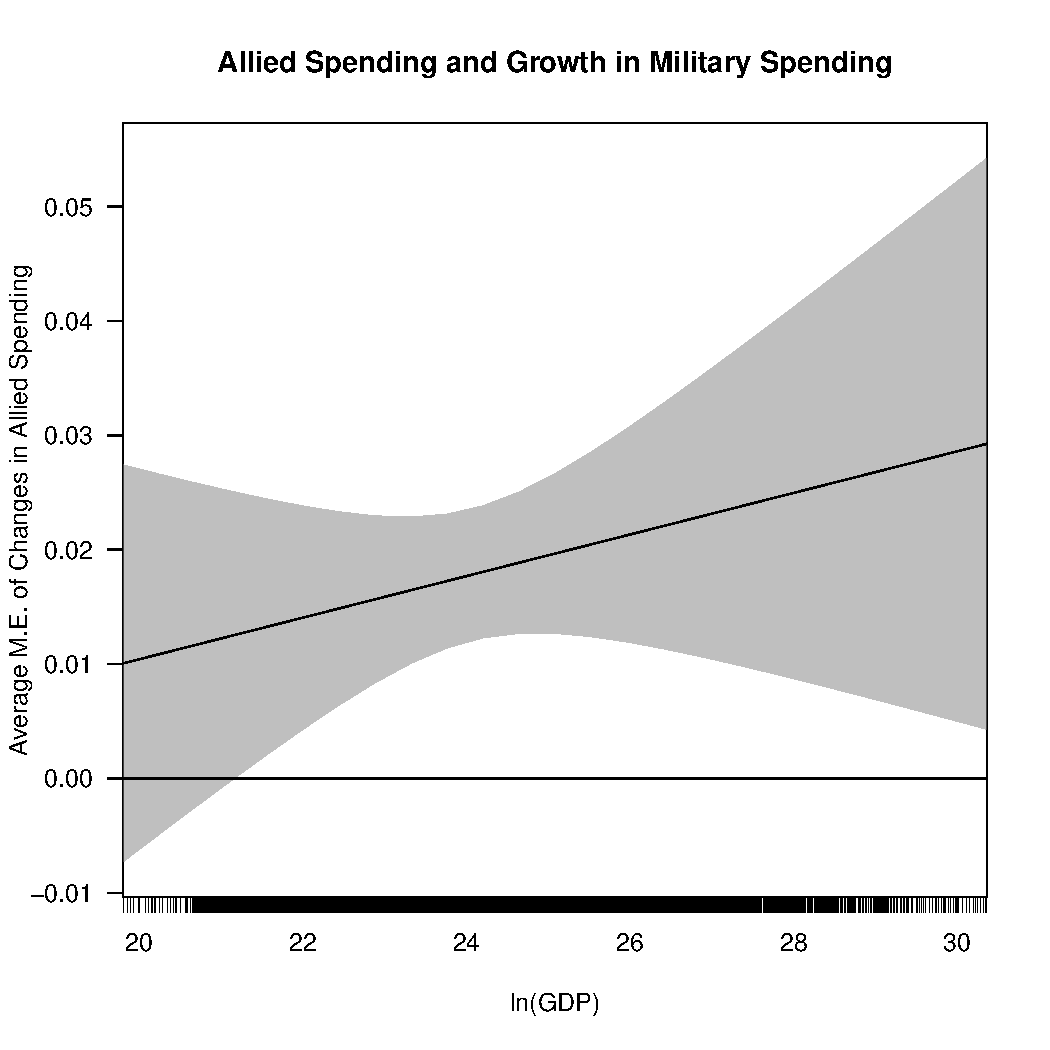
\includegraphics[width=0.95\textwidth]{abs-margins-plot.pdf}
	\caption{Average marginal effect of increasing allied military spending on growth in military spending across the range of GDP. Rug plot on x-axis summarizes the distribution of GDP.}
		\label{fig:abs-margins-plot}
\end{figure}



I draw similar conclusions from a wide range of estimation strategies, and report all those results in the appendix.\footnote{One of those checks is estimates the model with OLS instead of robust regression.}
Because the modifying variable is continuous, I employ kernel estimation of the interactive relationship \citep{Hainmuelleretal2019}.
Another check uses a robust regression estimator with random effects for states and years \citep{Koller2016}. 
I also transform the military spending growth variable using an inverse hyperbolic sine to reduce the heavy-tails in positive and negative values, and used the transformed variable in OLS and robust regressions. 


These results do not match the expectations of Hypothesis 1. 
The point estimate is uniformly positive and although the confidence intervals include negative values at very small levels of GDP, the effect of increasing allied capability is reliably positive for most of the range of GDP. 
There is little evidence that increasing allied capability decreases growth in spending for small states. 


However, it is possible that this aggregate analysis obscures variation across individual treaties. 
Exploitation may be more obvious by comparing spending growth within alliances. 
The next section tests Hypothesis 2 by examining how many treaties have a positive correlation between economic contribution and growth in military expenditures. 


\section{Testing Hypothesis 2}


Testing Hypothesis 2 requires estimating the association between alliance contribution and military spending within each alliance.
Unlike the test of Hypothesis 1, this process disaggregates alliances to examines relative state size. 
For each of the 285 alliances that promise military support,\footnote{ATOP offensive and defensive treaties. Other alliances do not provide security through promises of intervention in conflict. Thinking about the relative contribution to the aggregate capability of a non-aggression pact would be odd, for example.} 
I estimate a parameter measuring the impact of increasing alliance contribution on military expenditures. 
Bayesian estimation regularizes estimates with many parameters, so I fit the following model using STAN \citep{Carpenteretal2016}.


The model starts with state-year growth in military spending $y_{it}$.
I model this outcome with a t-distribution to account for heavy tails.
$\nu$ is the degrees of freedom parameter--- as $\nu$ increases, the t distribution becomes more like a normal distribution. 


\begin{equation}
y_{it} \sim student_t(\nu, \mu_{it}, \sigma) 
\end{equation}


Most of this model follows standard panel data designs.
The expected value of the outcome $\mu_{it}$ depends on a constant $\alpha$, state and year varying intercepts $\alpha^{st}$ and $\alpha^{yr}$ and control variables $X_{it} \beta$. 
In this specification, I include all controls besides the alliance portfolio averages from the test of Hypothesis 1 in $X$.


\begin{equation}
\mu_{it} = \alpha + \alpha^{st} + \alpha^{yr} + \mathbf{X_{it}} \beta + \mathbf{Z_{it}} \gamma 
\end{equation}


The $\mathbf{Z_{it}} \gamma$ term captures the impact of multiple alliances. 
\textbf{Z} is a matrix of state participation in alliances--- columns are alliances, rows are state-year observations. 
If a state is not in an alliance, the corresponding element of the matrix is equal to zero. 
If a state is part of an alliance, the corresponding element of the matrix is equal to a state's GDP as a share of total GDP in the alliance.\footnote{All GDP values are logged.} 
The elements of \textbf{Z} range between zero and one. 


\textbf{Z} is a quasi-spatial approach to capturing the impact of participation in multiple alliances.
The ``weight'' of an alliance for growth in military spending depends on the relative economic resources a state contributes.  
As a state's share of total allied GDP increases, so does its potential military spending contribution to allied security.  
According to the exploitation hypothesis, greater treaty contribution will increase demand for military spending. 
Smaller states will have lower growth in spending, because they can free-ride on their partners.
Thus, alliance participation impacts military spending through economic contribution. 
This correlation between treaty contribution and growth in spending for each alliance is expressed in the $\gamma$ parameters. 


$\gamma$ is a vector of 285 alliance-specific parameters.  
Because \textbf{Z} contains alliance contribution, these coefficients estimate the association between treaty contribution and military spending. 
When a state is not in an alliance, the corresponding $\gamma$ is multiplied by zero, and has no impact. 


Each alliance a state is a member of has a separate impact on military spending.
While these alliance parameters are distinct, they are related through partial pooling--- they have a common prior distribution.
Partial pooling estimates the dispersion of the alliance parameters from the data, so the prior for $\gamma$ is normally distributed with mean $\theta$ and variance $\sigma_{all}$. 
$\theta$ is the mean hyperparameter of the alliance coefficients, so each alliance parameter deviates from that value.
The extent of those deviations from $\theta$ depend on the variance hyperparameter $\sigma_{all}$.
Every alliance estimate holds the impact of other treaties constant. 
A positive $\gamma$ implies that alliance members with higher economic contribution have higher growth in military spending, as Hypothesis 2 predicts. 
    


\subsection{Results} 


If the public goods theory of alliances is correct, we should observe many positive $\gamma$ parameters. 
Because I employed Bayesian modeling, each $\gamma$ has a posterior distribution.\footnote{See the appendix for a full summary of priors, convergence and model fit. I also show that the model can recover known parameters from simulated data.} 
I focus interpretation on the posterior mean and 90\% credible intervals.\footnote{I use 90\% credible intervals because inferences around 95\% intervals can be less stable.}
The posterior mean is the expected value of $\gamma$, while the credible intervals capture uncertainty around that estimate.  


\begin{figure}[htbp]
	\centering
		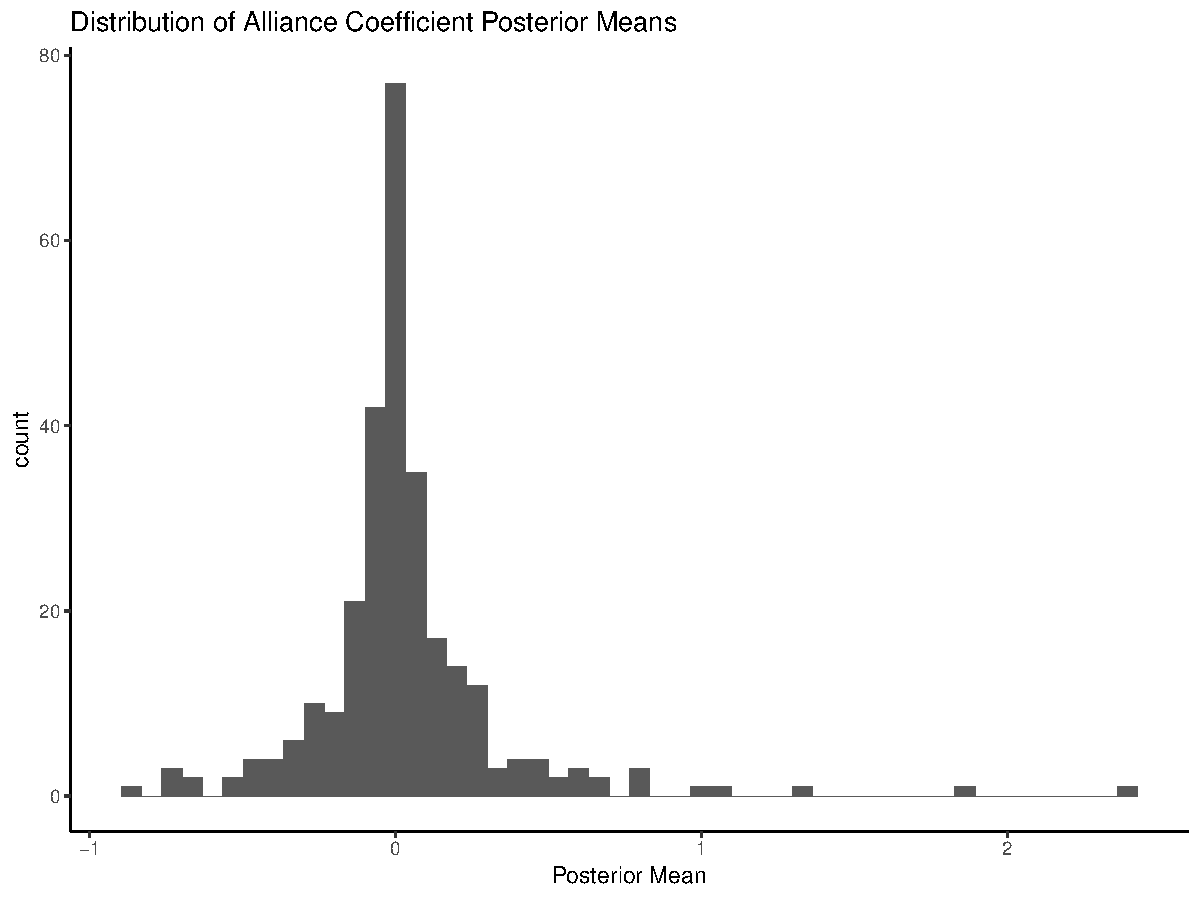
\includegraphics[width=0.95\textwidth]{alliance-coefs-hist.pdf}
	\caption{Posterior mean of association between alliance contribution and military spending in 285 defensive and offensive alliances from 1816 to 2007.}
	\label{fig:alliance-coefs-hist}
\end{figure}


\autoref{fig:alliance-coefs-hist} summarizes the posterior mean of the 285 alliance coefficients. 
Most means are close to zero. 
All 285 alliances have a negative posterior mean. 
This alone is evidence against Hypothesis 2. 


However, the posterior means do not convey the full range of possible effects. 
Positive mass in the posterior of the $\gamma$ parameters matches Hypothesis 2. 
\autoref{fig:full-post-prob} plots the relative positive and negative posterior probability of each $\gamma$ parameter. 


\begin{figure}[htbp]
	\centering
		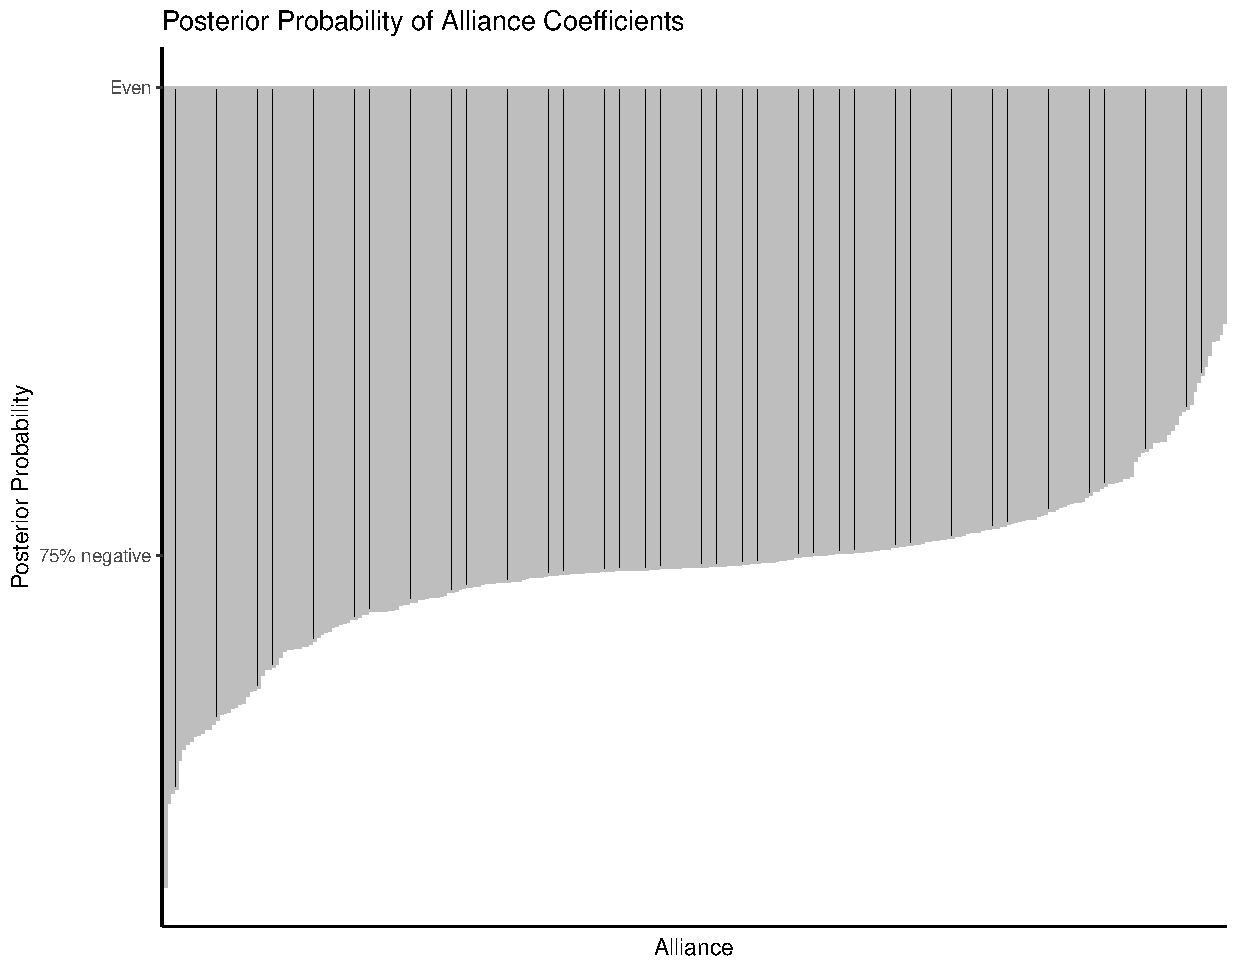
\includegraphics[width=0.95\textwidth]{full-post-prob.pdf}
	\caption{Positive and negative posterior probability of $\gamma$ parameters, sorted by posterior mean. Each column corresponds to an alliance and expresses the relative positive or negative posterior probability. Even posterior probability implies 50\% positive and negative posterior mass--- a $\gamma$ parameter with mean 0 and perfectly symmetric uncertainty. Deviations from this add positive or negative posterior mass.}
	\label{fig:full-post-prob}
\end{figure}


In all 285 alliances, the majority of the posterior mass is negative.  
Three alliances have 37\% positive posterior mass, and all other treaties are more negative. 
There is no alliance where the preponderance of evidence suggests that greater treaty contribution increases military spending. 


The credible intervals of each $\gamma$ parameter are another source of information about the likely effect of treaty contribution.\footnote{The 90\% credible interval falls between the 5\% and 95\% quantiles of the posterior.} 
These intervals help determine if the correlations between the share of allied GDP and growth in military spending can be distinguished from zero. 
\autoref{fig:alliance-coefs-year} plots the $\gamma$ parameter for each alliance against the start year of the treaty.
Points mark the posterior mean. 
The error bars encapsulate the 90\% credible interval.


\begin{figure}[htbp]
	\centering
		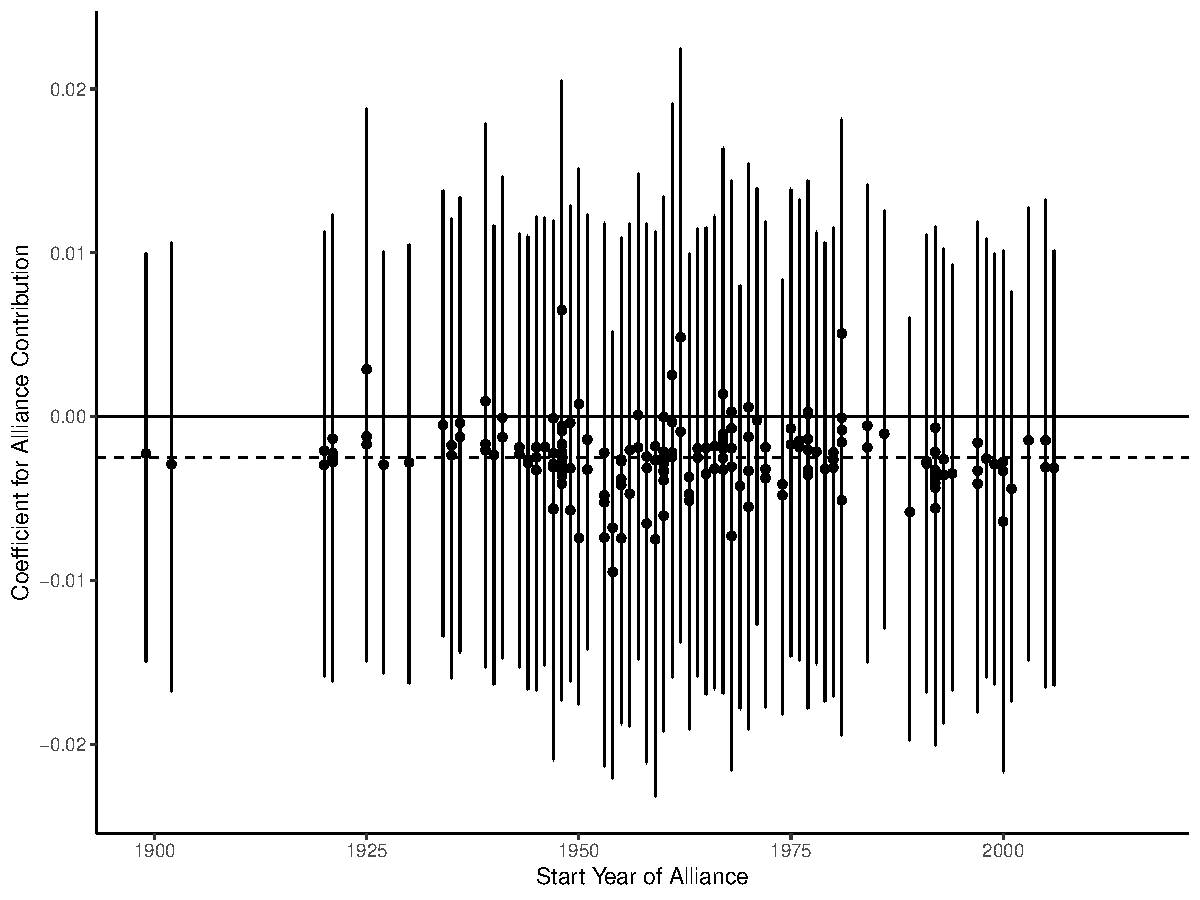
\includegraphics[width=0.95\textwidth]{alliance-coefs-year.pdf}
	\caption{Estimated association between alliance contribution and defense spending in 285 defensive and offensive alliances from 1816 to 2007. Points represent the posterior mean and the error bars cover the 90\% credible interval. The dashed line marks the posterior mean of the $\theta$ parameter, which estimates the average effect of increasing treating contribution on growth in military spending.}
	\label{fig:alliance-coefs-year}
\end{figure}


All 285 credible intervals include zero. 
As such, there is little evidence treaty contribution impacts military spending. 
No approach to examining the association between GDP as a share of allied GDP and military expenditure shows a preponderance of positive coefficients. 
Most alliances have no clear association between treaty contribution and growth in military spending.


As \autoref{fig:alliance-coefs-year} shows, partial pooling of the $\gamma$ parameters strongly regularizes these estimates. 
$\theta$ has a posterior mean of -0.006, which is close to zero. 
The variance hyperparameter $\sigma_{all}$ has a posterior median of 0.01. 
As a result, the data indicates that the effects of increasing treaty contribution $\gamma$ are tightly clustered around the overall mean. 
Under these circumstances, it will be very difficult to distinguish any estimates from zero, even as partial pooling shares strength across coefficients and reduces uncertainty. 


The $\gamma$ estimates allow for inferences about individual alliances, so I now highlight a few noteworthy cases. 
One alliance has greater than 90\% negative posterior probability: a 1972 pact between Hungary and Romania (ATOPID 3680). 
Several other bilateral alliances among Warsaw Pact members have large negative posterior means (ATOPID 3605 and ATOPID 3610). 

 
The estimated $\gamma$ for NATO offers no support for the public goods theory of alliances. 
The posterior mean is $-0.01$, and the credible interval ranges from -.03 to .01.  
Greater contribution to the total GDP of NATO has no clear association with growth in military spending. 
This finding corroborates the results of \citet{PluemperNeumayer2015}.\footnote{But it does not rule out the possibility that NATO members spend less on the military thanks to allied capability, which a great deal of evidence suggests is the case \citep{GeorgeSandler2017}. Instead, it shows that greater economic contribution has an unclear impact on NATO members military spending.}


In summary, this test of the second hypothesis turns up minimal evidence smaller alliance members have lower growth in military spending due to treaty participation. 
Instead all treaties have a negative mean association between an increasing share of alliance GDP and growth in military spending. 
Few treaties have a preponderance of evidence for a positive or negative correlation between economic contribution and growth in expenditures.  
 


\section{Conclusion}

% Add paragraph summarizing results
Taking the results from testing Hypothesis 1 and 2 together, there is little evidence for the prediction of the public goods theory of alliances that small alliance members are able to exploit their partners. 
I do not find that economic size modifies the impact of alliance participation on growth in military spending.
Moreover, there is no clear association between treaty contribution and military spending. 
No matter how it is expressed, the exploitation hypothesis that smaller states are able to spend less on the military through free-riding on allies has scant support. 


These findings should increase our skepticism about the public goods model of alliances. 
Although Olson and Zeckhauser's model is parsimonious, it lacks explanatory power. 
Better identified empirical models and estimates from multiple treaties show little evidence to match predictions from a public goods logic. 


My results reinforce theoretical skepticism about the public goods model. 
While I have shown little general evidence of collective action problem, pieces of the public goods model may still be useful. 
Critiques by \citet{Palmer1990} and \citet{SandlerHartley2001} merit further attention, but scholars should be cautious about using modified public goods models. 


A plausible theoretical alternative to the public goods approach emphasizes exchange between alliance members and intra-alliance bargaining \citep{Norrlof2010, Brooksetal2013, Kim2016}. 
Perhaps large and small states use alliances for distinct purposes, so members reap specific gains from treaty participation \citep{Morrow1991, Johnson2015}. 
Small states might use alliances to defend their homeland. 
Large states could be more focused on using alliances to defend other states and expand their influence abroad. 


Scholars and policymakers should reassess the way they use ``free-riding'' to describe alliance politics. 
Free-riding is inextricable from a public goods understanding of alliances.
But if key predictions of the public goods model have little empirical support, free-riding is an inaccurate description of reduced defense effort by alliance participants.  
Again, charges of free-riding may mask exchange between alliance members \citep{Lanoszka2015}. 
Junior partners in an alliance may still lower defense spending, but this reflects exchange, not exploitation. 
Larger partners also benefit from alliance participation when exchange occurs. 


Though policymakers may still find free-riding rhetoric useful, the idea is charged. 
Substantial anecdotal evidence suggests people dislike being taken advantage of. 
Talk of free-riding and exploitation could activate these concerns and undermine the alliance itself.
Policymakers might undermine support for alliances by accusing allies of free-riding. 


Scholars should not abandon the public goods model in international politics. 
Other international organizations such as environmental regimes and climate change suffer from clear collective action problems.  
Using alliances as exemplars of collective action problems in other international organizations is inappropriate, however. 


Although influential, the public goods model of alliances does not make accurate predictions about state size, allied capability and defense spending. 
Thinking about alliances through exchange may be more fruitful than the collective action problem envisaged by Olson and Zeckhauser.
Policymakers and scholars should exercise caution in using to the public goods model to understand alliance politics.  



\singlespace


\bibliography{../../../MasterBibliography} 





\end{document}

